% UIC Thesis Template by
% Michele Spagnuolo - http://michele.spagnuolo.me
% Feb 2013

\documentclass[letterpaper,11pt,oneside,final]{uicthesis}
\usepackage{amsfonts, amsmath, amsthm, amssymb, epsfig, graphicx, float}
\usepackage[longnamesfirst,square,sort&compress, comma, super]{natbib}
\usepackage[xindy,style=index]{glossaries}
\usepackage{bera}
\usepackage{lipsum}\usepackage{lipsum}

% Configuration
	% Thesis title
	\newcommand{\thesisTitle}{Thesis Title}
	% Thesis author
	\newcommand{\thesisAuthor}{Gabriele Petronella}
	% Author's previous degrees
	\newcommand{\authorDegrees}{B.S., Politecnico di Milano, July 2011}
	% Current degree (Thesis's degree)
	\newcommand{\thesisDegree}{Master of Science in Computer Science}

\usepackage[unicode,
			pdftex,
			plainpages=false,
			linktoc=all,
			hyperindex,
			breaklinks=true,
			citecolor=green,
			urlcolor=blue
		   ]{hyperref}
\hypersetup{
	pdftitle={\thesisTitle},
	pdfauthor={\thesisAuthor}
}

% Style
% !TEX root =  ../thesis.tex

\usepackage[top=43mm, bottom=44mm, left=41mm, right=32mm]{geometry}

\def\chapterautorefname{Chapter}
\def\sectionautorefname{Section}
\def\subsectionautorefname{Section}
\def\subsubsectionautorefname{Section}
\def\figureautorefname{Figure}
\def\tableautorefname{Table}

% Double spacing for text
\linespread{1.3}
% No square brackets in bibliography
\makeatletter
\renewcommand\@biblabel[1]{#1.}
\makeatother
% Bibliography style
% \renewcommand\bibname{}
% \renewcommand{\bibsection}{\section*{}}
% Single spacing list of abbreviations
% \renewcommand*{\glsgroupskip}{}
% Hyperref fix
\def\texorpdf #1#2{\texorpdfstring{#1{#2}}{#2}}

\usepackage[Lenny]{fncychap}

% Acronyms (to appear in the List of Abbreviations)
\makeglossaries
% !TEX root =  ../thesis.tex

% \newacronym{SMT}{SMT}{Simultaneous MultiThreading}
% \newacronym{OS}{OS}{Operating System}
% \newacronym{CPU}{CPU}{Central Processing Unit}
% \newacronym{I/O}{I/O}{Input/Output}
% \newacronym{GUI}{GUI}{Graphical User Interface}
% \newacronym{GPLv2}{GNU GPLv2}{GNU General Public License (version 2)}
% \newacronym{PID}{PID}{Process IDentifier}
% \newacronym{RSDL}{RSDL}{Rotating Staircase Deadline Scheduler}

\begin{document}
	\title{\huge{\thesisTitle}}
	\author{\thesisAuthor}
	\pdegrees{\authorDegrees}
	\degree{\thesisDegree}
	\maketitle

	\dedication
		% !TEX root =  ../thesis.tex
\setcounter{page}{2}

\begin{flushright}
	\emph{To my family} \\
\end{flushright}

	\acknowledgements
		% !TEX root =  ../thesis.tex

I want to thank Prof. Lenore D. Zuck for all the support and time she dedicated to me, helping me through this whole thesis work.
Then, I would like to thank want to tank Prof. Robert H. Sloan for the time he spent helping me in refining the scope of this thesis work.
Another thanks goes to Prof. Stefano Zanero for assisting me with his precious advice.

I finally want to thank all the people who shared with me this wonderful study and life experience in Chicago. I learned from this people more that I could ever possibly learn from books. Thank you for you awesomeness.

\begin{flushright}
GP
\end{flushright}


	% Optional Preface
	% \preface \label{preface}
	%	Blah
	
	\tableofcontents
	\listoftables
	\listoffigures
	% Remember to run makeglossaries thesis
		\glsaddall
		\printglossary[title=LIST OF ABBREVIATIONS]

	\summary \label{summary}
		Summary\ldots

	\chapter{Introduction} \label{chap:intro}
		% !TEX root =  ../thesis.tex

%%%%%%%%%%%%%%%%%%%%%%%%%%%%%%%%%%%%%%%%%%
During the last few years, mobile applications constantly grew in both number and importance in our everyday life. 

% \todo[inline]{Statistical data about mobile applications and device owners}

Such an impressive growth is marking a technology revolution, and, as many revolutions, it carries huge consequences affecting everyone's life. Some of these consequences lead to clear improvements, whereas others put under the spotlight some concerns that were not that relevant just a few years ago.

The increase in penetration and capabilities of mobile devices has turned them in something most people would find hard to separate from. Mobile devices nowadays typically hold a huge amount of information about their owners: email, messages, contacts, bank accounts, social network profiles, location information.

% \todo[inline]{Third-party applications}

How and under which circumstances such information can be disclosed has quickly become a concern.


This thesis work focuses on the first two steps discussed in the previous section.

The first step requires an in-depth analysis and comprehension of the most requested permissions, in order to identify the potential privacy concerns each one of them carries.

Once the permissions of interest have been identified we then perform a manual analysis in order to understand how privacy policies deal with the privacy concerns represented by them. The manual analysis will enable an automated process, which, given an arbitrary Android application published on the Play Store platform, retrieves its privacy policy and produces a human-readable report about the relationships between the permissions list and the analyzed legal document.

The final result will then allow a potential user to aggregate a large amount of privacy-related information in a quick and concise way, marking a clear step towards privacy awareness.

%%%%%%%%%%%%%%%%%%%%%%%%%%%%%%%%%%%%%%%%%%

The remainder of this thesis is organized as follows. Chapter 2 presents the manual analysis performed over privacy policies and permissions. Chapter 3 then describes the automatic analysis of Android apps, enabled by the results of Chapter 2. Chapter 4 presents the details of the implementation and of the tools used to support both manual and automated analysis. Chapter 5 presents a metric used for evaluating the compliance of Android applications w.r.t. their privacy policies, as well as quantitative results - measured with such metric - and qualitative results. Chapter 6 concludes this thesis, proposing possible further developments to the work done.
	\chapter{State of the Art} \label{chap:SOA}
		% !TEX root =  ../thesis.tex
\section{Privacy awareness context}
We now define the scope of this thesis, going through the main factors affecting privacy in mobile applications, and describing the existing relationships between them.

We identify three main factors to take into consideration:
\begin{itemize}
  \item permissions
  \item actions and behaviors
  \item privacy policies
\end{itemize}

\emph{Permissions} determine which data or services the app can access on the user's device, so they effectively define the maximum potential impact an application can have over the user's privacy: the fewer the permissions, the lower the risk. However, a recent study \cite{stickley} showed how, given only the \texttt{INTERNET} permission, an Android application was capable of stealing online account login credentials.
This highlights how permissions only represent a loose upper bound to the risk: even apps requesting one single permission can significantly affect the privacy of user.

% As discussed in \autoref{sec:android-permission-model}, permissions are declared upfront by Android applications and they are visible prior to the app's installation.

We define \emph{actions} as the minimum unit of work an application can do. Actions can be divided in two main categories

\begin{itemize}
  \item actions that cannot be performed without an explicit permission, and actions
  \item that do not require such explicit permission (e.g. impact local state of app)
\end{itemize}
The former category typically includes actions that have any impact on the device's security. Such actions are forbidden by the OS (\emph{Operating System}) by default, and are allowed only if specific permissions have been granted to the application. The latter usually represents actions not affecting the device's security, e.g. actions confined within the bounds of the application's internal logic.

We define \emph{behaviors} as sequences of one or more actions; such definition implies that some behaviors, namely those including actions from the first category, can occur only when specific permissions have been granted.


\begin{example}
\leavevmode
Let us a consider a game application that stores user's top scores and sends them over the Internet to a remote server.
We can break this app down into the following actions:
\begin{itemize}
  \item \texttt{save\_user's\_top\_scores} ($A_1$)
  \item \texttt{send\_top\_scores\_over\_the\_internet} ($A_2$)
\end{itemize} 
The sequence of $A_1$ and $A_2$ forms the behavior \texttt{store\_and\_send\_user's\_ top\_score\_to\_a\_ remote\_sever} ($B_1$).
$A_2$ requires the permission \linebreak \texttt{INTERNET} to be granted, whereas $A_1$ can always be performed.
This implies that $B_1$ can occur only if permission \texttt{INTERNET} is granted.
\end{example}

Thus, permissions enable actions, and actions can be composed to form behaviors. It is important to notice the cardinality of these relationships: one permission enables one or more actions; in turn, a behavior is enabled by one or more actions.

A many-to-many relationship exists between permissions and behaviors. Enabling one (or more) permissions can potentially enable one or more behaviors.
While some of these behaviors are expected, and even desirable, some others might result unexpected and potentially undesirable. 

\begin{figure}[tb]
\centering
     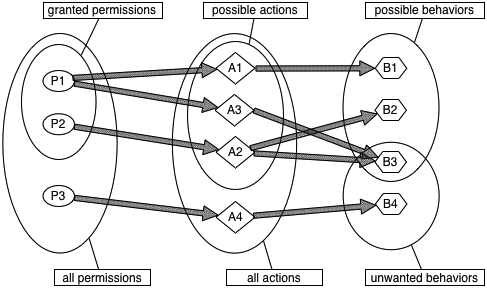
\includegraphics[width=0.9\textwidth]{images/context}
      \caption{Relationships between permissions, actions and behaviors}
      \label{fig:privacy-context}
\end{figure}

\autoref{fig:privacy-context} exemplifies this possible scenario: permission $P_1$ is required to enable action $A_1$ which in turn enables behavior $B1$. Similarly, permission $P_2$ enables action $A_2$ and consequently behavior $B_2$. Granting permissions $P_1$, however, also enables action $A_3$, and when combined with action $A_2$, an unwanted behavior $B_3$ may occur.

A practical instance of this scenario is the following:
\begin{example}
\leavevmode
\label{ex:unwanted-behavior}
\begin{itemize}
  \item the \texttt{READ\_PHONE\_STATE} permission enables the action \texttt{detect\_an\_ incoming\_phone\_call} ($A_1$), which enables the behavior \texttt{pause\_ the\_game\_when\_an\_incoming\_phone\_ call\_arrives} ($B_1$).
  \item the \texttt{INTERNET} permission enables the action \texttt{\justify send\_and\_receive\_ data\_over\_the\_Internet} ($A_2$), which enables the behavior \texttt{send\_ the\_user's\_top\_score\_to\_a\_remote \_server} ($B_2$).
  \item the \texttt{READ\_PHONE\_STATE} permission also enables the action \texttt{read\_the\_ user's\_phone\_ number} ($A_3$). The combination of actions $A_2$ and $A_3$ enables the behavior \\ \texttt{send\_the\_user's\_phone\_number\_to\_a\_remote\_server}($B_3$), which may be undesirable.
\end{itemize} 
\end{example}

Since the permission-based model has such shortcomings in properly restricting actions and avoiding unwanted behaviors, privacy policies are commonly provided together with the application, acting as a supplementary filter on the possible behaviors, telling the final users which of the possible behaviors the app is going to actually generate.

Coming back to Example 2, a privacy policy may explicitly state that the user's phone number is never collected nor accessed, promising the application will never perform \emph{A3}, and hence ruling out \emph{B3}. Nonetheless, nothing forbids an app to deviate from its policy.

\section{Scope of this thesis}
This thesis work focuses on the first two steps discussed in the previous section.

The first step requires an in-depth analysis and comprehension of the most requested permissions, in order to identify the potential privacy concerns each one of them carries.

Once the permissions of interest have been identified we then perform a manual analysis in order to understand how privacy policies deal with the privacy concerns represented by them. The manual analysis will enable an automated process, which, given an arbitrary Android application published on the Play Store platform, retrieves its privacy policy and produces a human-readable report about the relationships between the permissions list and the analyzed legal document.

The final result will then allow a potential user to aggregate a large amount of privacy-related information in a quick and concise way, marking a clear step towards privacy awareness.

%%%%%%%%%%%%%%%%%%%%%%%%%%%%%%%%%%%%%%%%%%

\section{Scope and goals of this thesis}
This thesis describes a methodology, supported by tools, that enables a user who installs an Android application to gain a better understanding of the app's capabilities, based on the permissions it requires and its privacy policy, and alerts the user to some of the (potentially) unintended consequences that the user grants the application by installing it.

\todo[inline]{Blablabla}
\section{Steps towards privacy awareness}
Given the general context of privacy awareness, we now identify a set of steps we intend to follow in our work, aiming at producing an increased users' awareness.

\begin{enumerate}
  \item Understanding permissions \hfill \\
    Previous studies \cite{Felt:2012:APU:2335356.2335360} show how permissions are rarely understood by users. Specifically users appear not be able to correlate a permission with the possible actions it enables, let alone the spectrum of possible behaviors derived from actions interleaving.

    The first step towards awareness is to analyze permissions and derive potential consequences. We are especially interested in permissions that directly affect privacy. As an example, the \texttt{READ\_PHONE\_ STATE} permission is typically requested by apps in order to be able to respond to phone events such as a incoming call, but it also enables the app to read the user's phone and IMEI numbers.

    Once permissions have been fully analyzed, one can then identify their  effect on the user's privacy.

  \item Correlating permissions and privacy policies \hfill \\
    The next step towards privacy awareness is to map each permission the app requests into its impact, as stated in its privacy policy.
    While privacy policies do not share a common defined structure, they do express similar concepts in similar ways, which allows us to extracting useful pieces of information from them. For example, an application requesting the \texttt{ACCESS\_FINE\_LOCATION} permission is very likely to be associated to a privacy policy containing expressions such as \emph{``GPS'', ``Location Services'', `Global Positioning System', etc}.

    This step takes into consideration each permission that enables an app to affect the user's privacy, with the final goal of building a dictionary of common expressions and patterns that associate the permission to natural language sentences in the privacy policy.

  \item Correlating apps behavior and privacy policies \hfill \\
    The final step is to monitor the app's actual behavior. Recalling Example \ref{ex:unwanted-behavior}, the application might never retrieve the user's phone number even though it requested such permission.

    On this basis we can advise the users about how well an application with respects the claims expressed in the privacy policy, and the actual actions taken by the app once installed and running on their phone.
\end{enumerate}

\begin{figure}[tb]
\centering
     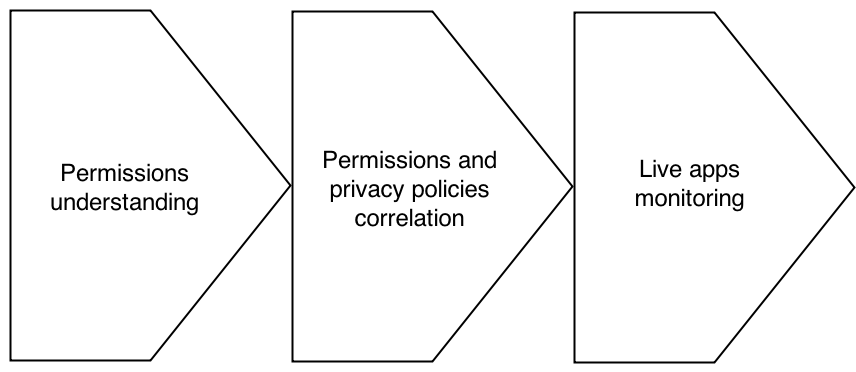
\includegraphics[width=0.8\textwidth]{images/awareness-steps}
      \caption{Privacy awareness steps}
      \label{fig:awareness-steps}
\end{figure}

%%%%%%%%%%%%%%%%%%%%%%%%%%%%%%%%%%%%%%%%%%

\section{Android OS Permission Model}
\label{sec:android-permission-model}
As explained in the Android Developer Guide, ``Android is a privilege-separated operating system, in which each application runs with a distinct system identity. [...]
Additional finer-grained security features are provided through a permission mechanism that enforces restrictions on the specific operations that a particular process can perform, and per-URI permissions for granting ad-hoc access to specific pieces of data. [...]
A basic Android application has no permissions associated with it by default, meaning it can not do anything that would adversely impact the user experience or any data on the device.''\cite{android-developer-guide}.
In order to access the protected features of the device the developer has to declare a list of permissions the application needs. This list is specified in the \texttt{AndroidManifest.xml}, a file containing application metadata, included by every Android application.

For example, an application that needs to send and receive data over the Internet would specify an \texttt{AndroidManifest} similar to the one in \autoref{lst:manifest}.

\begin{lstlisting}[
caption=Example of permission declaration in AndroidManifext.xml,
language=XML,
backgroundcolor=\color{white},
label=lst:manifest,
frame=single,
float,
basicstyle=\ttfamily\footnotesize
]
<manifest xmlns:android="http://schemas.android.com/res/android"
    package="com.example.anapp" >
    <uses-permission android:name="android.permission.INTERNET"/>
    ...
</manifest>
\end{lstlisting}

``At application install time, permissions requested by the application are granted to it by the package installer, based on checks against the signatures of the applications declaring those permissions and/or interaction with the user.
No checks with the user are done while an application is running: it either was granted a particular permission when installed, and can use that feature as desired, or the permission was not granted and any attempt to use the feature will fail without prompting the user.''\cite{android-developer-guide}

%%%%%%%%%%%%%%%%%%%%%%%%%%%%%%%%%%%%%%%%%%
\section{Related Work}
As discussed in \autoref{sec:android-permission-model}, permissions are granted at install time, meaning that a user is supposed to have reviewed the permissions the application requested and to have deemed them acceptable, before granting them altogether.

Such mechanism has been criticized for several reasons: first of all, recent studies \cite{Felt:2012:APU:2335356.2335360} \cite{Kelley:2012:CPI:2426020.2426027} show how users might not have complete understanding of the meaning and consequences of each permission in the list. The same studies also show how even experienced users are found not to pay attention to the permission list, most likely due to its verbosity and length. To further prove this last observation, in a recent experiment \cite{stickley} an ad-hoc application was developed and put on the Play Store; the application requested all possible permissions, enabling the researchers to steal personal data from the user, such as email addresses and phone numbers. The application received 1300 downloads over a 3-month period, without being advertised, and collected 1950 email addresses.

%%%%%%%%%%%%%%%%%%%%%%%%%%%%%%%%%%%%%%%%%%
	\chapter{Proposed Approach} \label{chap:approach}
		\input{chapters/approach}
	\chapter{Proposed Implementation} \label{chap:implem}
		% !TEX root =  ../thesis.tex
In this chapter we present the details of the implementation. We first describe the data collection process, for privacy policies and permissions; we then discuss how the collected data were subsequently analyzed, preprocessed and selected. Finally, we present the implementation of the algorithms discussed in the previous chapter.

%%%%%%%%%%%%%%%%%%%%%%%%%%%%%%%%%%%%%%%%%%
\section{Permissions collection}
\label{sec:permissions-collection}
As discussed in \autoref{sec:android-permission-model}, Android apps are required to declare upfront a list of all the permissions they need. Such list is stored in the \texttt{AndroidManifest.xml} file of each app. At installation time the user is able to review the permissions and decide whether to grant them or not.

Due to the lack of public official API for retrieving the permissions list, we first attempted to retrieve it through the Play Store web interface.

From a programmatic point of view, however, some issues arise. First of all, the permissions presented to the user are in a natural language format, whereas the permissions in the \texttt{AndroidManifest.xml} file are expressed with a canonical name. For instance the permission \texttt{READ\_ EXTERNAL\_STORAGE} correspond to the natural language description \emph{``modify or delete the contents of your USB storage''}.
This would require an extra processing step to map the natural language description back to the corresponding permission.

Secondly, and most importantly, the permission list is accessible from the web interface only after pressing the `install' button, and this step is allowed only from a registered Google account with at least one Android device registered.

While these issues can be overcome, they added unexpected complexity to this step, and therefore an alternative path was explored.

As mentioned above, Google does not provide an official API for retrieving applications metadata, such as the permission list. However an unofficial Python implementation exists and is publicly available \cite{play-store-unofficial-api}. There also exists another open-source project \cite{play-store-crawler}, based on the unofficial API, featuring the ability of performing search queries, downloading apps and retrieving apps permissions.

Thank to the use of the unofficial API, the issues mentioned above were solved and we were able to retrieve the permissions from an arbitrary app available on the Play Store.

%%%%%%%%%%%%%%%%%%%%%%%%%%%%%%%%%%%%%%%%%%
\section{Privacy Policy collection}
\label{sec:pp-collection}
Automatically retrieving a privacy policy document for an arbitrary Android app is a much harder task than retrieving its permission list.

Whenever present, the Privacy Policy link appears in the \emph{Additional Information} section on the Play Store web interface, as shown in \autoref{fig:play-store-privacy-link}.

\begin{figure}[tb]
\centering
     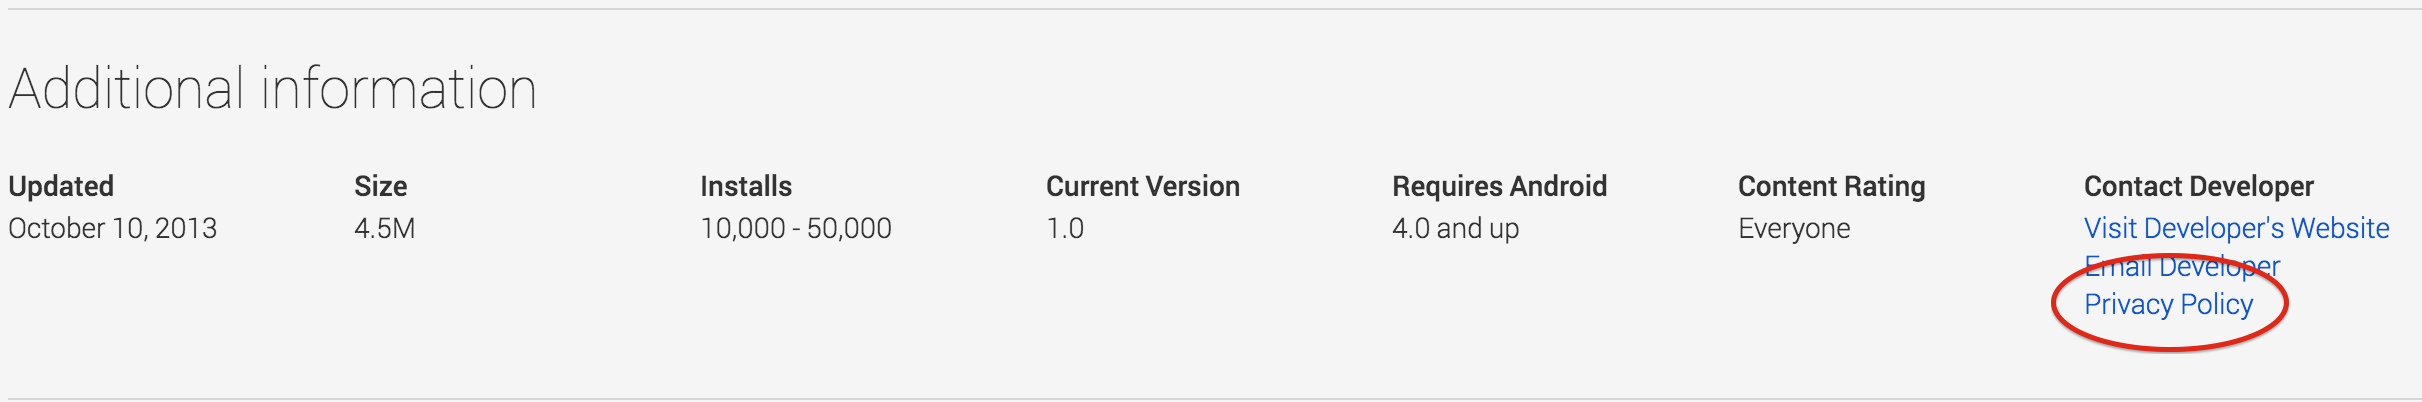
\includegraphics[width=\textwidth]{images/play-store-privacy-link}
      \caption{Privacy Policy link in the Play Store web interface}
      \label{fig:play-store-privacy-link}
\end{figure}

However, while the \texttt{AndroidManifest.xml} file is guaranteed to be present for any application on the Play Store, this does not hold true for the Privacy Policy link. 

In fact, no Play Store policies force an app to have a Privacy Policy at all.

So it can occur that either the app does not have a Privacy Policy at all, or that the developer has not inserted the Privacy Policy on the Play Store. In either case the automatic retrieval of the Privacy Policy of that app is impossible, so we will not further distinguish between them.

From the data we collected, it appears that out of the 1093 most downloaded free game apps, 39.79\% do not have a privacy policy publicly available through the Play Store.

% \todo[inline]{insert a pie chart here}

That being said, a Privacy Policy link does not guarantee the ability to retrieve an actual Privacy Policy document. The link can point to anything the developer decides, and this leads to extremely heterogeneous paths to reach the final document of our interest.

An example is redirection, which that is very common. As an example, the Privacy Policy URL for \emph{Angry Birds}, by Zynga, is:

\url{https://www.google.com/url?q=http://m.zynga.com/about/privacy-center/privacy-policy}

which redirects to

\url{http://m.zynga.com/about/privacy-center/privacy-policy}

which redirects to

\url{http://company.zynga.com/privacy/policy}

which contains the Privacy Policy document.

% \todo[inline]{Talk about the Disney example}

%%%%%%%%%%%%%%%%%%%%%%%%%%%%%%%%%%%%%%%%%%
\section{Semantic analysis}
Once the document has been retrieved, it needs to be semantically processed. For this purpose, we take advantage of Treat, a natural language processing framework for Ruby \cite{treat}. The Treat project aims to build a language-agnostic NLP framework for Ruby with support for tasks such as document retrieval, text chunking, segmentation and tokenization, natural language parsing, part-of-speech tagging, keyword extraction and named entity recognition.

The privacy policy document is firstly split into its logical subdivision using a SRX chunker, which implements the approach proposed in \cite{Milkowski:2009:USS:1987717.1987736}.

The the document is furthed split into sentences with the aid of a SRX segment, again following \cite{Milkowski:2009:USS:1987717.1987736}.


\begin{figure}[tb]
\centering
     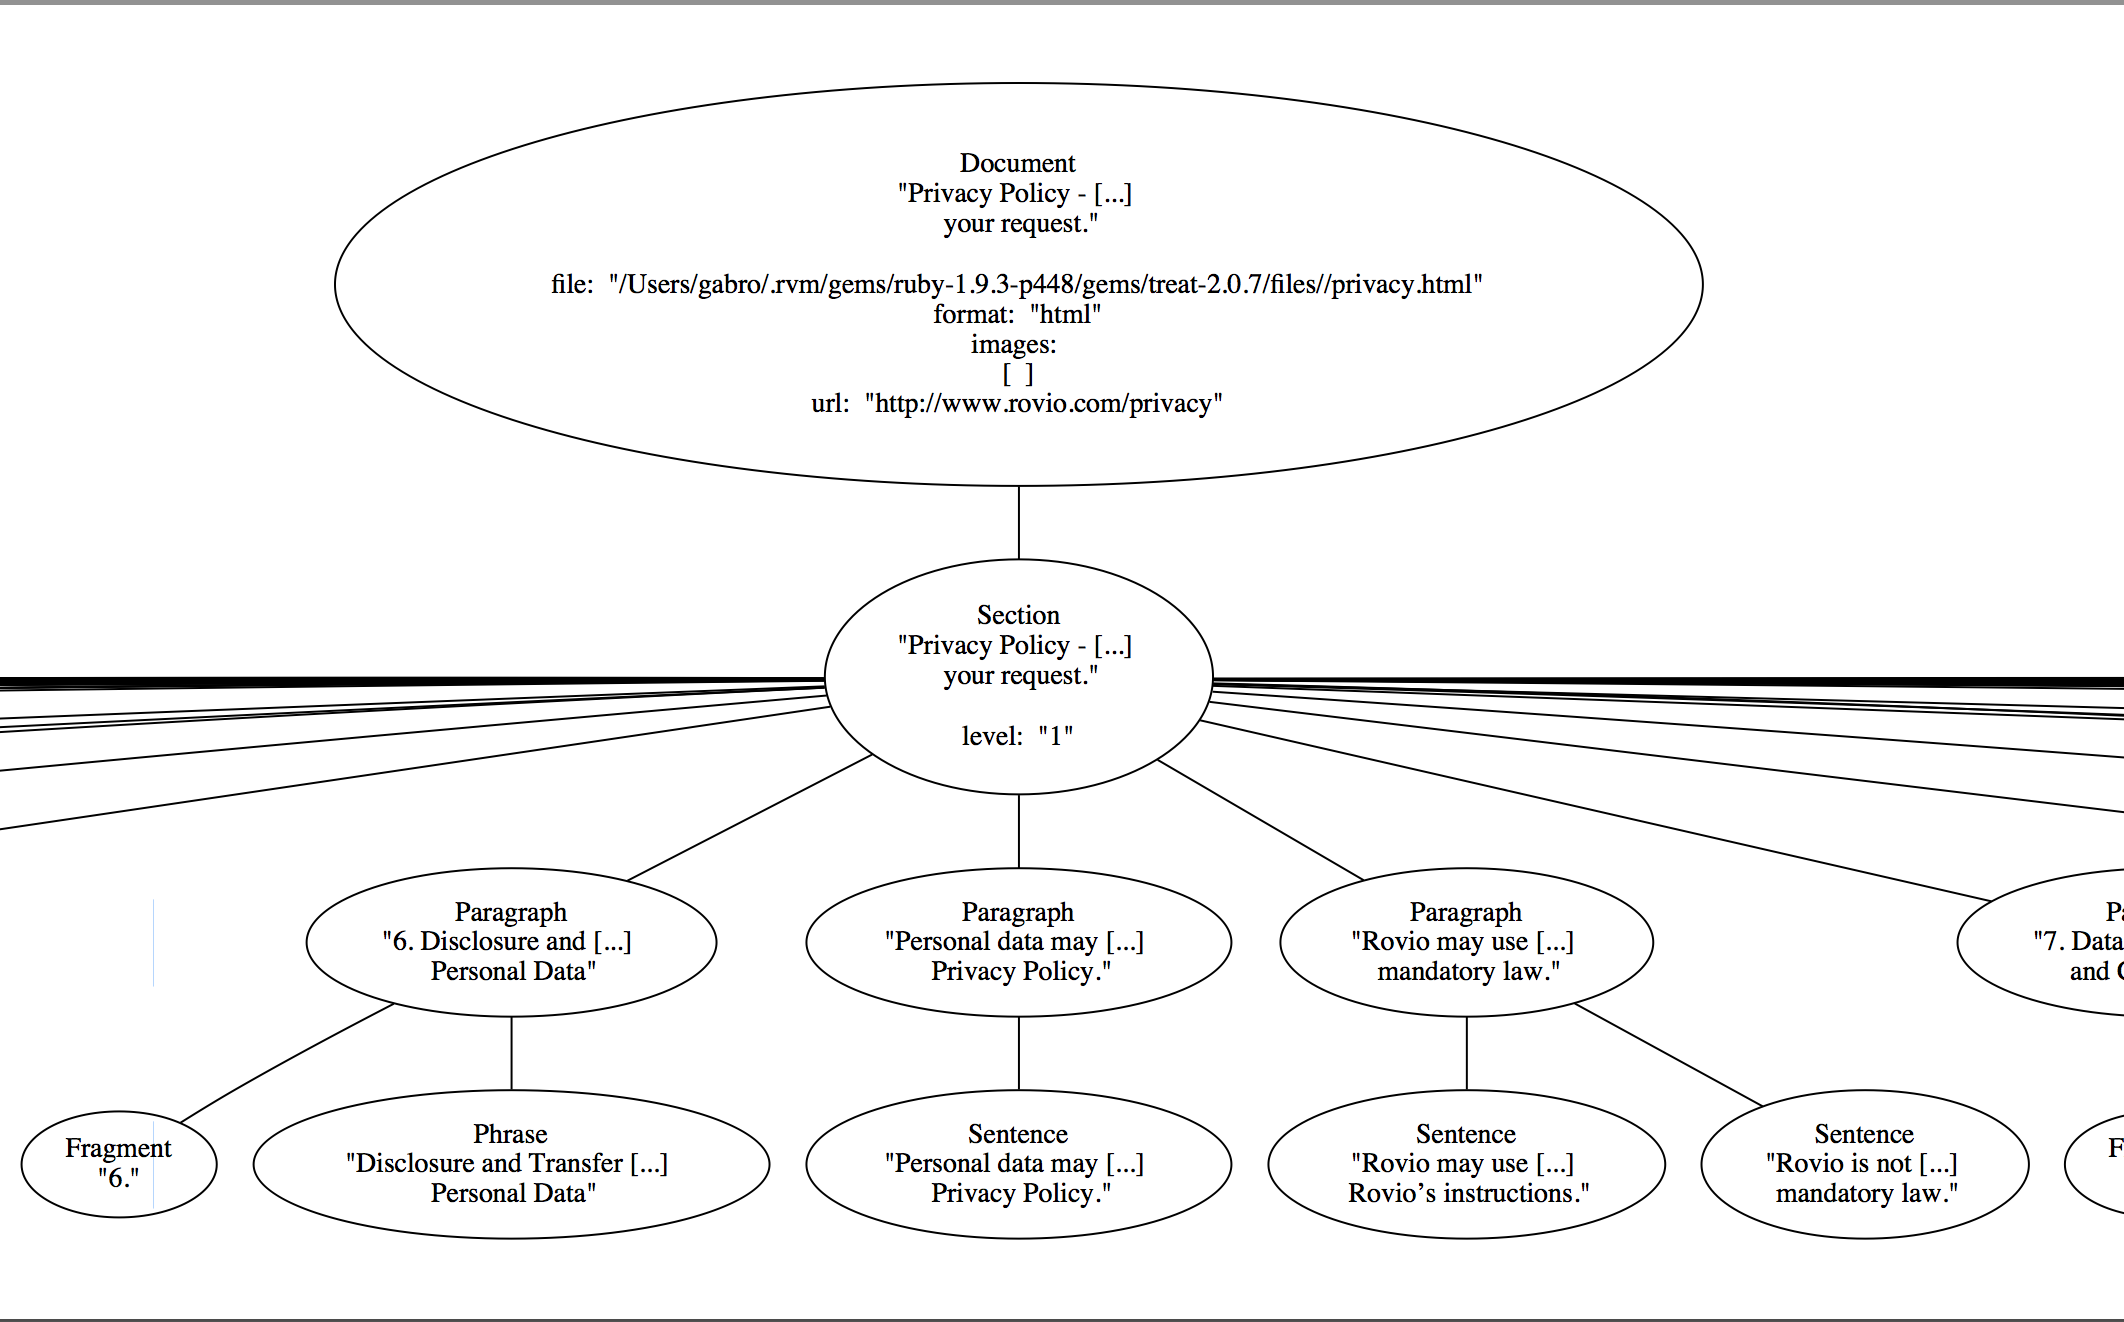
\includegraphics[width=\textwidth]{images/rovio-structure}
      \caption{Detail of Rovio's Privacy Policy structure}
      \label{fig:rovio-structure}
\end{figure}

\autoref{fig:rovio-structure} shows a detail of the semantic tree in which the original policy has been divided. Each internal node represents either paragraphs or sections of the document, whereas the leaf nodes are phrases and sentences.

Once sentences and phrases have been obtained, they can be searched for the expressions contained in the lookup table of each permission.
For example let us take the following sentence.

\begin{quote}
{\emph{``Rovio or third parties operating the ad serving technology may use demographic and \textbf{geo-location} information (for more information regarding use of Location Data see below Section 3) as well as information logged from your hardware or device to ensure that relevant advertising is presented within the Service.''}}\cite{rovio}
\end{quote}

The lookup table of \texttt{ACCESS\_COARSE\_LOCATION} contains the word ``location'', hence the above sentence will be matched and will be considered relevant to such permission.

\subsection{False positive detection}
As explained in \autoref{sec:false-positives}, we also need to search for `banned' verbal forms and exclude the sentences containing them. In order to be as general as possible, we want to consider every possible declination of the verb.
So the two main steps of this phase are:
\begin{itemize}
  \item identifying the verbs
  \item `normalizeing' each verb, in order to perform a comprehensive comparison
\end{itemize}

\subsubsection{Verb identification}
Identifying the verbs is achieved through \emph{part-of-speech tagging} (POS). POS, also called \emph{word-category disambiguation}, ``is the process of marking up a word in a text (corpus) as corresponding to a particular part of speech, based on both its definition, as well as its context—i.e. relationship with adjacent and related words in a phrase, sentence, or paragraph. A simplified form of this is commonly taught to school-age children, in the identification of words as nouns, verbs, adjectives, adverbs, etc.'' \cite{wiki:POS}. Different language taggers have been proposed over the last years: our choice fell on the most established one, i.e. the Stanford POS Tagger, which is a Java implementation of the log-linear POS tagger proposed in \cite{Toutanova:2003:FPT:1073445.1073478}.
Specifically we used the Ruby bindings provided by the aforementioned Treat framework.

As anticipated, the language tagger assigns a \emph{tag} to each word of a sentence; the tags used by the Standford Tagger are defined by the Penn Treebank tag set \cite{Marcus:1994:PTA:1075812.1075835}, in which we can find five different verb tags

\begin{itemize}
  \item VB:      Verb, base form
  \item VBD:     Verb, past tense
  \item VBG:     Verb, gerund or present participle
  \item VBN:     Verb, past participle
  \item VBP:     Verb, non-3rd person singular present
  \item VBZ:     Verb, 3rd person singular present 
\end{itemize}

Since we are interested in all the verbs of a sentence, we therefore consider all words with any of the above tags.

\subsubsection{Verbs normalization}
We are not really interested in the inflection of the verbs we are analyzing, rather we care about the concept they represent.
In order to catch all possible verbal forms, we make use of another feature of Treat: inflections. This feature allows us to perform a grammatical conjugation of an arbitrary verb.
Hence, we normalize all the verbs to their infinitive form before performing a comparison. For example, if we encounter a sentence containing the verb ``shipping'' and our ``false positive table'' includes the verb ``ship'', the sentence will be correctly excluded from the final result set.

\section{Results}
Results are discussed in detail in \autoref{sec:results}, however their collection brought up several technical challenges that required a rather sophisticated solution. The main issue is represented by the significant number of applications we want to analyze; for each one of them we need to retrieve their privacy policy, their permission list and then analyze such information.

The challenges then become:
\begin{itemize}
	\item Performing thousands of simultaneous requests to Play Store servers
	\item Performing thousands of simultaneous analysis on the same machine
\end{itemize}

The first challenge derives from Google's anti-bot protection, which results in an IP-ban in case of too many requests in a short amount of time.
The second challenges is instead an architectural limitation: spawning thousands of simultaneous computations easily hogs any personal computer's CPU, most likely leading to a system crash.

A naive approach to both challenges would be to serialize the operations, analyzing only one application at the time. However, considering an average processing time of 10 seconds per application, analyzing thousands of applications would require several hours of computation and such an architecture would not scale in case of an increased number of applications (e.g., if one would like to analyze a significant fraction of the Play Store).

What we want is then a fixed amount of computations running concurrently, in order to achieve a fast computation without hogging the computer's resources. We achieved this result taking a functional approach, namely utilizing Celluloid, a concurrent object oriented programming framework for Ruby.

Using Celluloid, we spawn a new computation for each thread - or in other terms, an \emph{actor} - which runs asynchronously and writes the results back to a MongoDB database. We use a fixed amout of actors, collectively referred to as a pool, in order to prevent the computation from using all of the computer resources, and also to prevent being banned from Google.
The result is a satisfying compromise between speed and available resources that allows to terminate the computation within reasonable time constraints.
	\chapter{Experimental Results} \label{chap:results}
		% !TEX root =  ../thesis.tex

In this chapter the results of our investigation are presented. We illustrate the quantitative results deriving from an automated analysis of several application on the Play Store; subsequently, we present a qualitative analysis and observation about the experiment.

\section{Quantitative results}
\label{sec:results}
In this section we present a metric used to evaluate the compliance of an application w.r.t. its privacy policy and we expose the quantitative results in terms of such metric.

\subsection{Metric definition}
\label{sec:metric}
First, we manually assign to each privacy-related permission a score from 1 to 3, representing the severity of its potential impact on the user's privacy, where 1 signifies a permission with low impact and 3 signifies a permission carrying a very high danger.

Such scores are defined by us, in accordance with observations and existing literature on permission analysis,
and are shown in \autoref{tab:permission-scores}.

\begin{table}[ht]
    \caption{PERMISSION IMPACT SCORES}
    \label{tab:permission-scores}
    \centering
    \begin{tabular}{clc}
        \toprule
            \#   & Permission impact scores \\
            \midrule
                1  & INTERNET                       &   3 \\
                2  & READ\_EXTERNAL\_STORAGE        &   2 \\
                3  & WRITE\_EXTERNAL\_STORAGE       &   2 \\
                4  & ACCESS\_WIFI\_STATE            &   1 \\
                5  & READ\_PHONE\_STATE             &   3 \\
                6  & GET\_ACCOUNTS                  &   3 \\
                7  & ACCESS\_COARSE\_LOCATION      	&   3 \\
                8  & GET\_TASKS                     &   1 \\
                9  & ACCESS\_FINE\_LOCATION         &   3 \\
                10 & READ\_LOGS                     &   1 \\
                11 & RECORD\_AUDIO                  &   2 \\
                12 & READ\_CONTACTS                 &   3 \\
        \bottomrule
    \end{tabular}
\end{table}

Secondly, we use the scores to compute a weighted sum of the number of permissions that lack an explicit mention in the privacy policy.

\begin{align}
\label{eq:goodness-metric}
	\sum\limits_{i=1}^n &= w_i p_i \\
	w_i &= \text{ score of the} i^{th} \text{permission} \\
	%
	p_i &=
	\begin{cases}
		& 0 \text{ if the permission is mentioned in the privacy policy} \\
		& 1 \text{ otherwise}
	\end{cases}
\end{align}

The final result is a metric estimating the compliance of an Android application to its own privacy policy. The lower the score, the more compliant the application.

We the analysis on the same 4300 applications used to generate the list of most used permissions, and the results are shown in \autoref{fig:results}

\begin{figure}[t]
\centering
     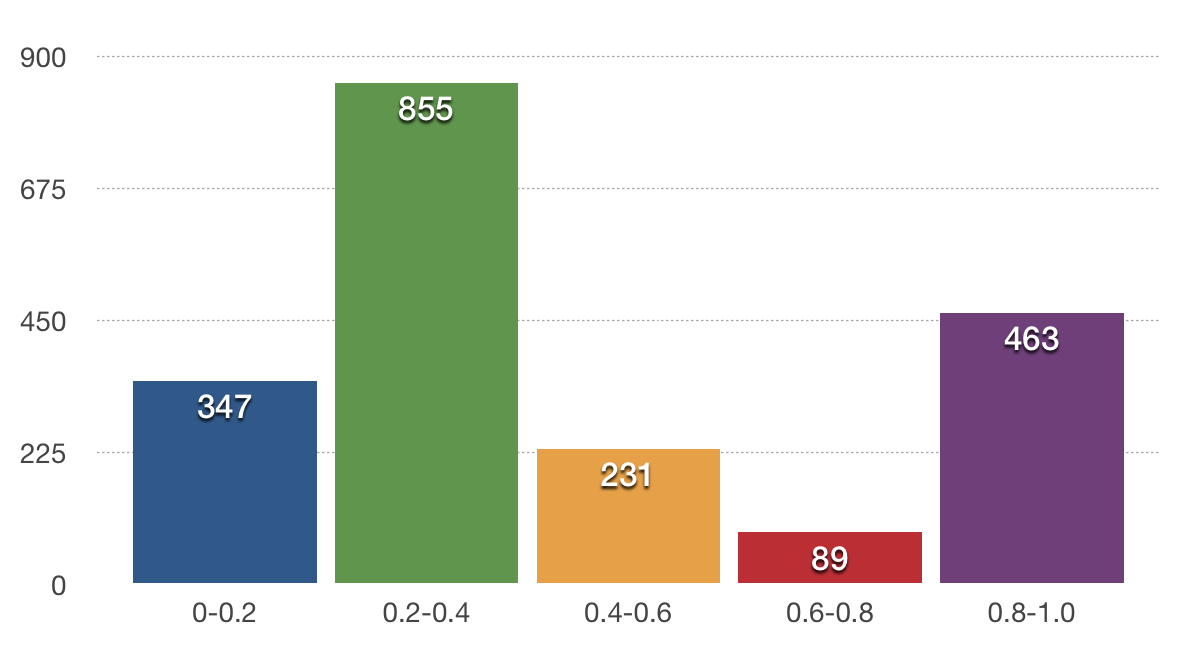
\includegraphics[width=0.9\textwidth]{images/results}
      \caption{Quantitative results (over 4300 applications, December 7, 2013)}
      \label{fig:results}
\end{figure}

\section{Qualitative results}
\label{sec:qualitative-results}
Out of the thousands of applications analyzed, we now focus our attention on a few notable cases.

\section{Case study: Shopkick}
Shopkick is a popular shopping rewards app and is known \cite{shopkick-lifehacker} to require some sensitive permissions that should worry any user of this app. \autoref{tab:shopkick-permissions} shows the complete list of permissions of the Android application.

\begin{table}[ht]
    \caption{SHOPKICK APP PERMISSIONS}
    \label{tab:shopkick-permissions}
    \centering
    \begin{tabular}{l}
        \toprule
            Permissions \\
            \midrule
                INTERNET \\
                ACCESS\_NETWORK\_STATE \\
                ACCESS\_COARSE\_LOCATION \\
                ACCESS\_FINE\_LOCATION \\
                READ\_PHONE\_STATE \\
                WRITE\_EXTERNAL\_STORAGE \\
                ACCESS\_WIFI\_STATE \\
                RECORD\_AUDIO \\
                CAMERA \\
                FLASHLIGHT \\
                VIBRATE \\
                BLUETOOTH \\
                GET\_ACCOUNTS \\
                RECEIVE\_BOOT\_COMPLETED \\
                READ\_CONTACTS \\
                CALL\_PHONE \\
                WAKE\_LOCK \\
                READ\_EXTERNAL\_STORAGE \\
                READ\_CALL\_LOG \\
        \bottomrule
    \end{tabular}
\end{table}

We can immediately spot a few permissions with a very high impact score, for example \texttt{RECORD\_AUDIO}, \texttt{CAMERA} and \texttt{ACCESS\_FINE\_LOCATION}.

\texttt{RECORD\_AUDIO} grants the application the ability to access the device microphone to record audio, without any explicit consent by the user other than installing the app itself. This means that the app is virtually enabled to record audio at any time, with no possibility of being disabled. Especially in combination with the \texttt{RECEIVE\_BOOT\_COMPLETED} permission, which allows the app to be launched when the phone has booted, and the \texttt{INTERNET} permission, which enables sending data over the Internet, this is considerably worrying: the application could easily start itself as soon as the phone has been turned on, constantly record any sound going through the device's microphone and finally send everything over the Internet to a remote server, where the content can be stored and accessed in a later time.

To make things worse, the application also requests the permission \texttt{ACCESS\_FINE\_LOCATION}, meaning that the audio recording can be triggered according to the user's location, perhaps the workplace, home or other sensitive locations.

It is not hard to see how these capabilities can turn the app into a roving spyware, i.e. an application with whose hidden purpose is eavesdropping and spying on the device owners, as well as the people they have contacts with.

Further investigations reveal how the app apparently uses the device's microphone in order to validate the physical location of the user in a store. According to the New York Times, \emph{``The app knows someone is in a store by listening for an audio transmitter placed in each participating store; the phone's microphone picks up the signal, which people cannot hear.''}\cite{shopkick-nyt}.

We can formalize a subset of this situation in terms of the representation previously discussed in \autoref{chap:intro}.
\begin{itemize}
    \item The permission \texttt{RECORD\_AUDIO} ($P_1$) enables the action \\ \emph{record\_audio\_from\_the\_device\_microphone} ($A\_1$);
    \item the permission \texttt{INTERNET} ($P\_2$) enables the action \\ \emph{send\_data\_over\_the\_internet} ($A\_2$);
    \item the permission \texttt{CAMERA} ($P\_3$) enables the action \\ \emph{record\_images\_from\_the\_device\_camera} ($A\_3$);
    \item the permission \texttt{ACCESS\_FINE\_LOCATION} enables the action \\ \emph{detect\_location\_of\_device} ($A_4$)
\end{itemize}

The combination of $A_1$ and $A_2$ enables the behavior \emph{validate\_presence\_in\_store} ($B\_1$). On the other hand $A\_1$, $A\_2$, $A\_3$ and $A\_4$ can also be combined enabling the behavior \emph{record\_audio\_and\_video\_when\_user\_is\_at\_home} ($B_2$).

Both behaviors are unexpected to the user, but while $B_1$ is probably considered legit - and even desirable -, $B_2$ is definitely unexpected, undesirable, and possibly unlawful.

We now look at Shopkick's privacy policy looking for references of the aforementioned permissions.

\subsection{RECORD}
Our tool identifies this paragraph as relevant to the matter of recording audio:

\begin{quote}
{\emph{``(iv) record, determine or use information about or from another content delivery platform (for example, to unlock potential rewards or offers based on your watching of a specific a commercial or show that is broadcast on your television or on the web, the shopkick application may ask you to open the app while you are watching TV, and then \textbf{we may record or analyze the audio signal from the television set via the shopkick app and your cell phone's microphone}, to determine the commercial, and/or program, including the date and/or time)''}}\cite{shopkick}
\end{quote}

A manual inspection of the policy confirms that this is indeed the relevant section and that the permissions are covered by the privacy policy.

\subsection{ACCESS\_FINE\_LOCATION}
Concerning the user's location, the tool identifies this sentence as relevant:

\begin{quote}
{\emph{(i) automatically record information that your mobile phone/device sends or transmits, including […] geographical location (if you consent to that)}}
\end{quote}

While it is true that the privacy policy covers this matter, it is also worth noting how the last phrase is misleading: as we saw before, the user grants permissions at install time on an Android device, so the consensus has already been given. Stating \emph{If you consent to do that} gives a sense of false assurance.

\subsection{CAMERA}
The tool signals that no references have been found in the privacy policy regarding the \texttt{CAMERA} permission and a manual inspections confirms that Shopkick's privacy policy doesn't mention in any way the use of the device's camera as a medium of acquiring data.

As it currently stands, Shopkick's application can collect any image from the user's camera without they being notified and the privacy policy does not restrict this by any mean.

Our tool successfully detected this behavior, helping in identifying a gap in the privacy policy of this popular application.
	\chapter{Conclusions} \label{chap:conclusion}
		% !TEX root =  ../thesis.tex

We presented a novel approach to the analysis of privacy policies in the context of Android applications. We introduced a framework for reasoning and proving properties of privacy policies, laying down the foundation for a new area of investigation.

The tool we implemented greatly eases the process of understanding the privacy implications of installing third party apps and it has already been proven able to highlight worrisome instances of applications.

The tool is developed with expandability in mind, and further developments in the approach can easily be integrated in order to increase the reliability and effectiveness.

This thesis aims at laying the foundation for a new area of investigation, namely the relationship between mobile applications capabilities and behaviors and their privacy policies. As we mentioned in \autoref{chap:intro} several steps can be taken towards user awareness about privacy matters and this work covers the first necessary ones: identifying and analyzing the privacy-relevant permissions and examining their relationships with the privacy policies language. This enables further steps in the investigation and we now outline some of them.

As anticipated in \autoref{chap:intro}, the first natural steps following the present work would be to live monitor the application's behavior. A static analysis can provide useful information about the \emph{potential} behaviors that can occur, but only a dynamic observation of applications running on real device can give insights about the \emph{actual} behaviors.

The first implementation one can think of is a passive monitoring of applications, with the final purpose of reporting such behaviors and further refine the ``goodness'' score presented in \autoref{sec:metric}.

One can also think of taking a step further and turn the monitoring into an active defense: if the application is found performing a behavior clearly in contrast with its privacy policy, the monitoring tool can immediately inform the user or even prevent such behavior from happening.

As discussed in \autoref{sec:false-positives}, the proposed approachoccasionally incurs in false positives and we illustrated a possible solution to this issue based on verb detection.

As anticipated, another viable solution is to allow the users of the tool to provide feedback on each sentence. They could either mark the sentence as \emph{relevant} or \emph{not relevant} and therefore improve the scoring of an application.

The same approach could then be used to identify false negatives: relevant sentences can be not recognized and a user can signal such fact indicating which relevant portions of the privacy policy apply to the selected permission.

	\clearpage
	\phantomsection
	\appendices
		\appendix \label{app:a}
		% !TEX root =  ../thesis.tex
\begin{table}[tbh]
    \caption{ACCESS\_COARSE\_LOCATION LOOKUP TABLE}
    \label{tab:lookup-coarse-location}
    \centering
    \begin{tabular}{lp{6cm}}
        \toprule
            Permission   & Keywords \\
            \midrule
                \texttt{ACCESS\_COARSE\_LOCATION}  & \emph{``gps''}, \emph{``IP based location''}, \emph{``location''}, \emph{``location services''}, \emph{``geo-location''}, \emph{``geographic location''} \\
        \bottomrule
    \end{tabular}
\end{table}

\begin{table}[tbh]
    \caption{RECORD\_AUDIO LOOKUP TABLE}
    \label{tab:lookup-record-audio}
    \centering
    \begin{tabular}{lp{9cm}}
        \toprule
            Permission   & Keywords \\
            \midrule
                \texttt{RECORD\_AUDIO}  & \emph{``microphone''}, \emph{``record audio''}, \emph{``record voice''}, \emph{``audio''} \\
        \bottomrule
    \end{tabular}
\end{table}

	\clearpage
	\phantomsection
	\bib
	\bibliography{thesis}
	\nocite{*}

	\newpage
	\phantomsection

	% !TEX root =  ../thesis.tex
\vita

\begin{center}
\begin{singlespace}

{\Huge Gabriele Petronella}

\vspace{0.4in}

\begin{tabular}{r@{\hspace{0.2in}}|@{\hspace{0.2in}}p{3.8in}}

{\Large Education}
& \textbf{B.S., Engineering of Computing Systems} \\
& Politecnico di Milano \\
& 2011 \\
\\
& \textbf{M.S., Computer Science (\emph{current})} \\
& University of Illinois at Chicago, Chicago, IL \\
& 2013 \\
\\

{\Large Working experience}
& \textbf{Co-founder} \\
& \emph{Metwit Ltd}  \small{2011-2012}\\ 
& Dubai, UAE - London, UK \\
& Founded a crowdsourced weather startup and lead the develpment of the iOS client. \\
\\

& \textbf{Co-founder} \\
& \emph{buildo s.r.l.s.}  \small{2013-present}\\ 
& Milan, Italy \\
& Software architect and developer. \\
\\

& \textbf{Research Assistant} \\
& \emph{University of Illinois at Chicago} \small{Sept 2012-Dec 2013} \\
& Chicago, IL \\
& Research activity focused on privacy policies formal analysis.
\end{tabular}

\end{singlespace}
\end{center}

		\ldots
\end{document}
